\clearpage
\phantomsection

\setcounter{chapter}{4}

\chapter[{THỰC THI VÀ ĐÁNH GIÁ}]{thực thi và đánh giá}
Sau khi chứng minh được tính đúng đắn quá việc mô phỏng và kiểm thử , sinh viên sẽ thực hiện triển khai một hệ thống System on Chip để đánh giá về hiệu năng thực tế, đồng thời chứng minh IP đã thiết kế đảm bảo khả năng hoạt động với các thành phần khác.
\section{Thông tin về bo mạch Zynq UltraScale+MPSoC ZCU106 Evaluation Kit}
ZCU106 Evaluation Kit là bo mạch được phát triển để phục vụ mục đích thiết kế và tạo mẫu các hệ thống nhúng trên nền tảng của nhà sản xuất Xilinx. Nó là tổ hợp của hai phần gồm hệ thống xử lý (PS) và FPGA (PL). Với PL là hệ logic khả trình cho phép người dùng lập trình phần cứng để thực hiện các chức năng chuyên biệt, xử lý ... PS là ARM flagship Cortex-A53 64-bit quad-core processor và Cortex-R5F dual-core real-time processor. Ngoài ra trên bo mạch còn tích hợp rất nhiều các ngoại vi như HDMI, Ethernet, ...
\begin{figure}[!ht]
	\centering
	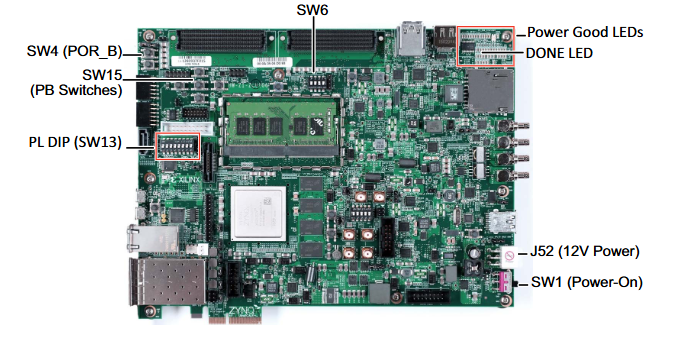
\includegraphics[width=1\linewidth]{figures/zcu106.png}
	\caption{Bo mạch ZCU106 UltraScale+MPSoC}
	\label{fig:zcu106}
\end{figure}
\section{Xây dựng hệ thống SoC}
Hình \ref{fig:soc1} mô tả về sơ đồ khối của hệ thống SoC sẽ được xây dựng. Ảnh có thể được lưu trữ trong DDR, sau đó DMA sẽ lấy dữ liệu ảnh trong DDR đó, chuyển vào khối IP. Vì có tín hiệu \textbf{start} để yêu cầu việc bắt đầu quá trình nên sẽ có một khối GPIO được điều khiển bởi PS để thực hiện bật, tắt chân start. Từ IP, một tín hiệu ngắt cũng sẽ được nối trở về PS để thực hiện thông báo ngắt khi cần. 
\begin{figure}[!ht]
	\centering
	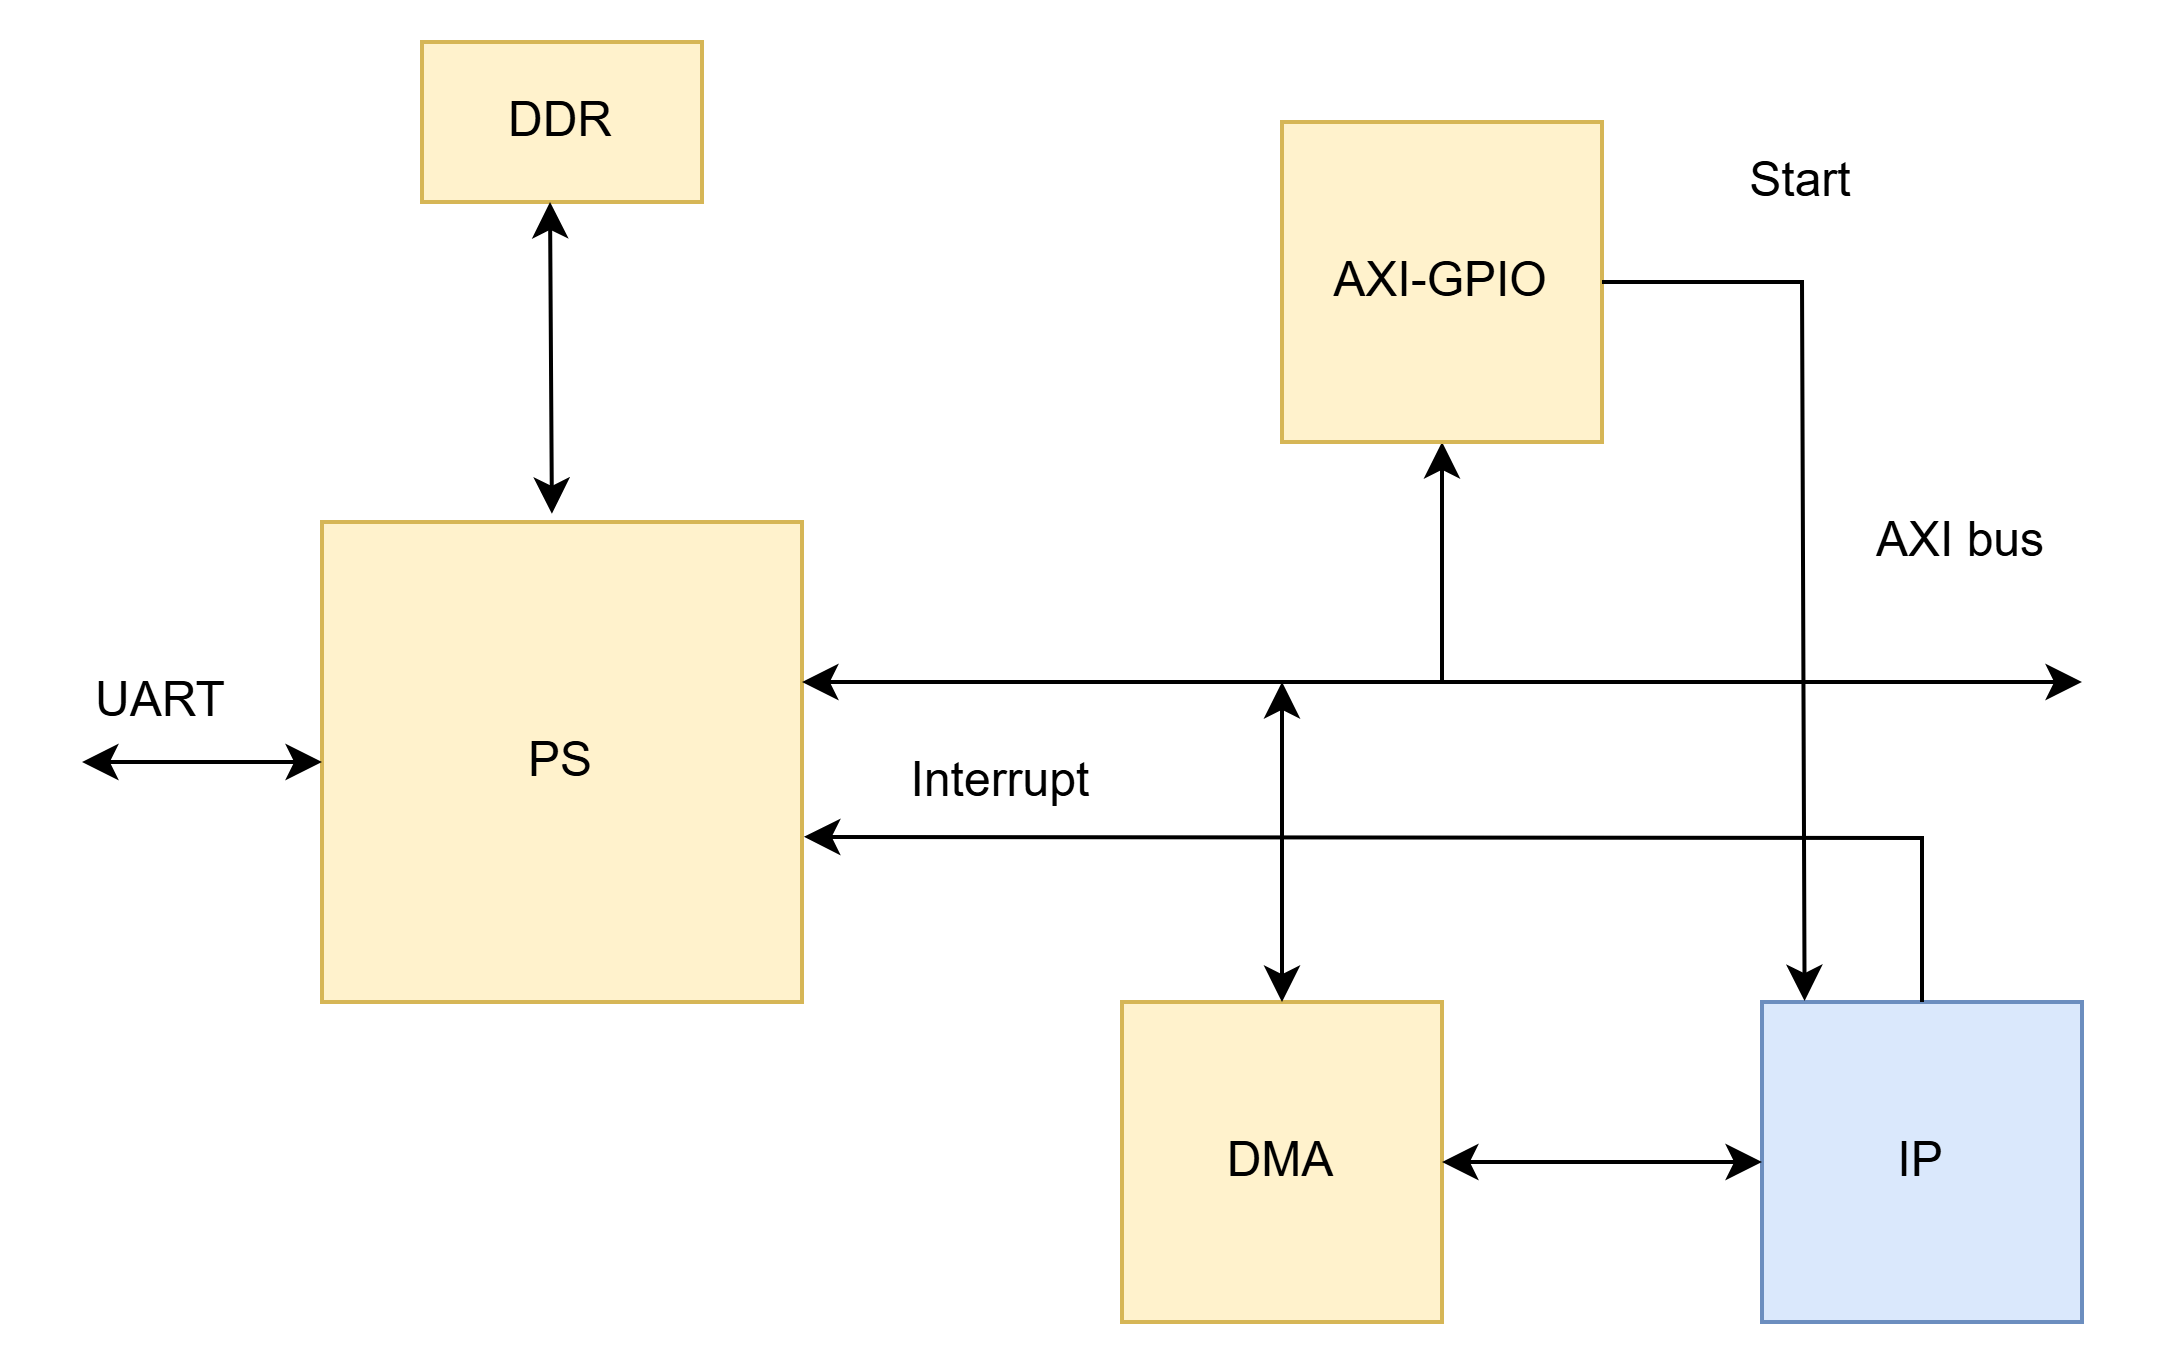
\includegraphics[width=0.6\linewidth]{figures/soc1.png}
	\caption{Sơ đồ khối hệ thống SoC}
	\label{fig:soc1}
\end{figure}
\section{Kết quả và đánh giá}
Kết quả về tổng hợp và thực thi sẽ được thực hiện trên phần mềm vivado 2018.2. Kết quả tổng hợp bao gồm về tài nguyên sử dụng, tần số tối đa, năng lượng tiêu thụ. Để đánh giá về độ chính xác của mô hình sẽ thực hiện với tập dữ liệu Outex, so sánh thời gian thực tế với thời gian chạy của các mô hình phần mềm.

Tài nguyên sử dụng được mô tả trong bảng \ref{tab:resoruce}

\begin{table}[H]
	\centering
	\renewcommand{\arraystretch}{1.3}
	\begin{tabular}{|p{2cm} p{2cm} p{2cm} p{2cm} p{4cm } p{2cm}|}
		\hline
		\rowcolor{gray!30}
		\textbf{Tài nguyên} & \textbf{Sử dụng}  & \textbf{Có sẵn} & \textbf{Phần trăm} &  \textbf{Wang,Zhang \cite{realTimeTexture}} & HLS  \\
		LUT & 20463 & 230400 & 8.88\% & 49033 & 1
		\\ \hline
		FF & 22559 & 460800 & 4.9\% & 19969 & 1
		\\ \hline
		BRAMs & 31.5 & 312 & 10.1\% & 41.5 & 1
		\\ \hline
	\end{tabular}
	\caption{Tài nguyên sử dụng}
	\label{tab:resoruce}
\end{table}


Thông số định thời của hệ thống được thể hiện trên hình \ref{fig:ipTiming}. Với các thông số định thời ta sẽ có một số tiêu chí đánh giá như sau:
\begin{itemize}
	\item WNS: Đỗ trễ trong trường hợp xấu nhất của một xung nhịp, WNS = $min(T-T_n)$ với T là một chu kỳ của xung nhịp, $T_n$ là thời gian truyền. Để mạch hoạt động chính xác thì phải đảm bảo giá trị WNS lớn hơn 0.
	\item Tần số $F_{max}$: Tần số có thể chạy trên phẩn cứng trong một triển khai nhất định.
\end{itemize}
Hệ thống được xây dựng với ràng buộc đầu là 100MHz tương đương với chu kỳ xung nhịp là 10ns, từ đó ta có thể tính tần số tối đa như sau:
\begin{equation*}
	F_{max} = \frac{1}{T - WNS} = \frac{1}{(10 - 4.918)*10^{-9}} = 196   (MHz) 
\end{equation*}

\begin{figure}[!ht]
	\centering
	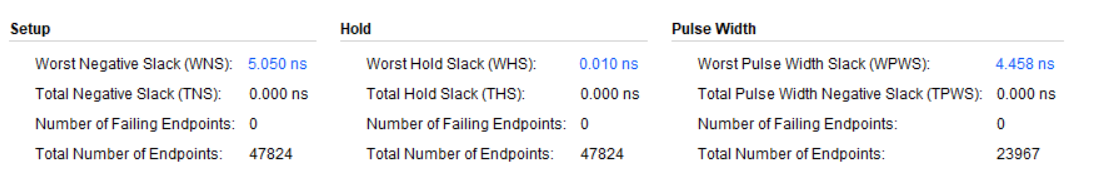
\includegraphics[width=\linewidth]{figures/ipTiming.png}
	\caption{Thông số định thời của IP}
	\label{fig:ipTiming}
\end{figure}

Công suất tiêu thụ của hệ thống được thể hiện trong hình \ref{fig:power}. Công suất tiêu thụ động là 0.595W bằng với công suất tiêu thụ tĩnh là 0.595W. Đây là mức tiêu thụ năng lượng không quá lớn để tích hợp với các hệ thống khác vì hoạt động của IP rất phức tạp và cần tối ưu về mặt đáp ứng thời gian thực.

\begin{figure}[!ht]
	\centering
	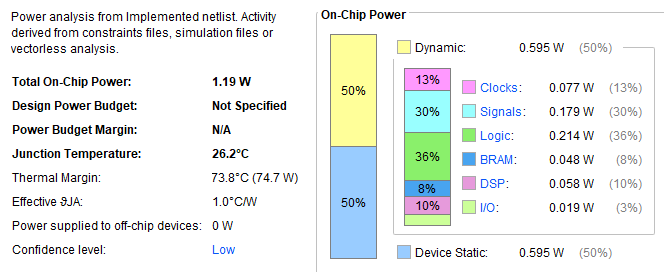
\includegraphics[width=\linewidth]{figures/power.png}
	\caption{Công suất tiêu thụ năng lượng của IP}
	\label{fig:power}
\end{figure}



\begin{table}[H]
	\centering
	\renewcommand{\arraystretch}{1.3}
	\begin{tabular}{|p{2cm} p{2cm} p{2cm} p{2cm} p{4cm } p{2cm}|}
		\hline
		\rowcolor{gray!30}
		\textbf{Tài nguyên} & \textbf{Sử dụng}  & \textbf{Có sẵn} & \textbf{Phần trăm} &  \textbf{Wang,Zhang \cite{realTimeTexture}} & HLS  \\
		LUT & 20463 & 230400 & 8.88\% & 49033 & 30378
		\\ \hline
		FF & 22559 & 460800 & 4.9\% & 19969 & 13713
		\\ \hline
		BRAMs & 31.5 & 312 & 10.1\% & 41.5 & 88
		\\ \hline
	\end{tabular}
	\caption{Bảng độ chính xác .... còn 1 số thông tin đang cần tính..}
	\label{tab:resoruce}
\end{table}


\section{Kết luận}
Căn cứ vào những kết quả đã đạt được, khóa luận đã đạt được những mục tiêu đề ra. Khóa luận đã cung cấp đầy đủ thông tin về kỹ thuật trích xuất đặc trưng với MRELBP, thiết kế phần cứng tăng tốc ở mức RTL và thiết kế hệ thống SoC kiểm chứng.  

Khóa luận đã hoàn thành các nhiệm vụ:
\begin{itemize}
	\item Phân tích, triển khai thuật toán MRELBP từ lý thuyết đã có
	\item Phân tích các yêu cầu, đưa ra thiết kế hệ thống ở mức RTL
	\item Xây dựng hệ thống SoC giúp kiểm chứng khả năng tương thiwhsc của IP
	\item Thực nghiệm, đánh giá kết quả thu được 
\end{itemize}}


Bên cạnh những điểm đã hoàn thành, đồ án vẫn tồn tại những nhược điểm lớn như công suất tiêu thụ năng lượng vẫn tương đối lớn và còn nhiều thiết kế chưa được pipeline một cách kỹ lương hơn. Đây là những thiết sót và cũng là những định hướng để cải tiến thiết kế trong tương lai.